\documentclass[10pt]{article}
\usepackage{tikz}
\usetikzlibrary{shapes.misc}
\usepackage[margin=0cm]{geometry}
\pagestyle{empty}
\tikzstyle{every node}=[cross out, draw, red]

\begin{document}

\vspace*{\fill}
\begin{center}
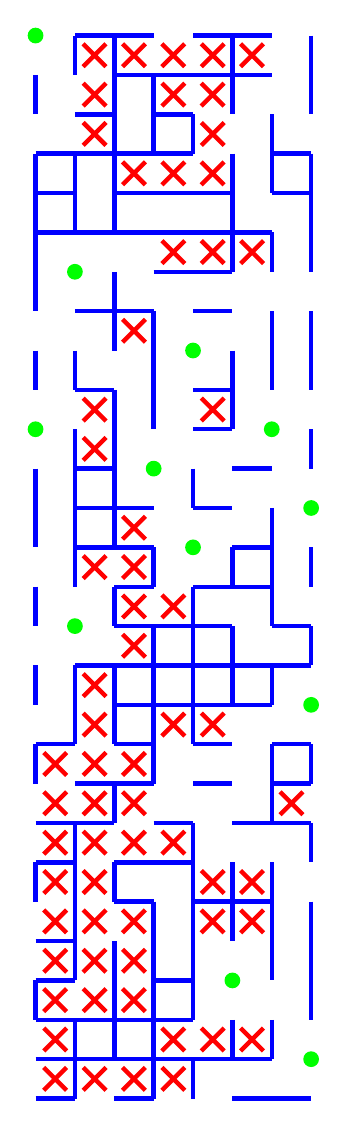
\begin{tikzpicture}[x=0.5cm, y=-0.5cm, ultra thick, blue]
% Walls
    \draw (1,0) -- (3,0);
    \draw (4,0) -- (6,0);
    \draw (2,1) -- (6,1);
    \draw (1,2) -- (2,2);
    \draw (3,2) -- (4,2);
    \draw (0,3) -- (4,3);
    \draw (6,3) -- (7,3);
    \draw (0,4) -- (1,4);
    \draw (2,4) -- (5,4);
    \draw (6,4) -- (7,4);
    \draw (0,5) -- (6,5);
    \draw (3,6) -- (5,6);
    \draw (1,7) -- (3,7);
    \draw (4,7) -- (5,7);
    \draw (1,9) -- (2,9);
    \draw (4,9) -- (5,9);
    \draw (4,10) -- (5,10);
    \draw (1,11) -- (2,11);
    \draw (5,11) -- (6,11);
    \draw (1,12) -- (3,12);
    \draw (4,12) -- (5,12);
    \draw (1,13) -- (3,13);
    \draw (5,13) -- (6,13);
    \draw (2,14) -- (3,14);
    \draw (4,14) -- (6,14);
    \draw (2,15) -- (5,15);
    \draw (6,15) -- (7,15);
    \draw (1,16) -- (7,16);
    \draw (2,17) -- (6,17);
    \draw (0,18) -- (1,18);
    \draw (2,18) -- (3,18);
    \draw (4,18) -- (5,18);
    \draw (6,18) -- (7,18);
    \draw (1,19) -- (3,19);
    \draw (4,19) -- (5,19);
    \draw (6,19) -- (7,19);
    \draw (0,20) -- (2,20);
    \draw (3,20) -- (4,20);
    \draw (5,20) -- (7,20);
    \draw (0,21) -- (1,21);
    \draw (2,21) -- (4,21);
    \draw (2,22) -- (3,22);
    \draw (4,22) -- (6,22);
    \draw (0,23) -- (1,23);
    \draw (0,24) -- (1,24);
    \draw (3,24) -- (4,24);
    \draw (0,25) -- (4,25);
    \draw (0,26) -- (6,26);
    \draw (0,27) -- (1,27);
    \draw (2,27) -- (3,27);
    \draw (5,27) -- (7,27);
    \draw (0,1) -- (0,2);
    \draw (0,3) -- (0,7);
    \draw (0,8) -- (0,9);
    \draw (0,11) -- (0,13);
    \draw (0,14) -- (0,15);
    \draw (0,16) -- (0,17);
    \draw (0,18) -- (0,19);
    \draw (0,21) -- (0,22);
    \draw (0,24) -- (0,25);
    \draw (1,0) -- (1,1);
    \draw (1,3) -- (1,5);
    \draw (1,8) -- (1,9);
    \draw (1,10) -- (1,14);
    \draw (1,16) -- (1,18);
    \draw (1,20) -- (1,24);
    \draw (1,25) -- (1,27);
    \draw (2,0) -- (2,5);
    \draw (2,6) -- (2,8);
    \draw (2,9) -- (2,13);
    \draw (2,14) -- (2,15);
    \draw (2,16) -- (2,18);
    \draw (2,19) -- (2,20);
    \draw (2,21) -- (2,22);
    \draw (2,23) -- (2,26);
    \draw (3,1) -- (3,3);
    \draw (3,7) -- (3,10);
    \draw (3,13) -- (3,14);
    \draw (3,15) -- (3,19);
    \draw (3,22) -- (3,27);
    \draw (4,2) -- (4,3);
    \draw (4,11) -- (4,12);
    \draw (4,14) -- (4,18);
    \draw (4,20) -- (4,25);
    \draw (4,26) -- (4,27);
    \draw (5,0) -- (5,2);
    \draw (5,3) -- (5,6);
    \draw (5,8) -- (5,10);
    \draw (5,13) -- (5,14);
    \draw (5,15) -- (5,17);
    \draw (5,21) -- (5,23);
    \draw (5,25) -- (5,26);
    \draw (6,2) -- (6,4);
    \draw (6,5) -- (6,6);
    \draw (6,7) -- (6,9);
    \draw (6,12) -- (6,15);
    \draw (6,16) -- (6,17);
    \draw (6,18) -- (6,20);
    \draw (6,21) -- (6,24);
    \draw (6,25) -- (6,26);
    \draw (7,0) -- (7,2);
    \draw (7,3) -- (7,6);
    \draw (7,7) -- (7,9);
    \draw (7,10) -- (7,11);
    \draw (7,13) -- (7,14);
    \draw (7,15) -- (7,16);
    \draw (7,18) -- (7,19);
    \draw (7,20) -- (7,21);
    \draw (7,22) -- (7,25);
% Pillars
    \fill[green] (0,0) circle(0.2);
    \fill[green] (1,6) circle(0.2);
    \fill[green] (4,8) circle(0.2);
    \fill[green] (0,10) circle(0.2);
    \fill[green] (6,10) circle(0.2);
    \fill[green] (3,11) circle(0.2);
    \fill[green] (7,12) circle(0.2);
    \fill[green] (4,13) circle(0.2);
    \fill[green] (1,15) circle(0.2);
    \fill[green] (7,17) circle(0.2);
    \fill[green] (5,24) circle(0.2);
    \fill[green] (7,26) circle(0.2);
% Inner points in accessible cul-de-sacs
    \node at (1.5,0.5) {};
    \node at (2.5,0.5) {};
    \node at (3.5,0.5) {};
    \node at (4.5,0.5) {};
    \node at (5.5,0.5) {};
    \node at (1.5,1.5) {};
    \node at (3.5,1.5) {};
    \node at (4.5,1.5) {};
    \node at (1.5,2.5) {};
    \node at (4.5,2.5) {};
    \node at (2.5,3.5) {};
    \node at (3.5,3.5) {};
    \node at (4.5,3.5) {};
    \node at (3.5,5.5) {};
    \node at (4.5,5.5) {};
    \node at (5.5,5.5) {};
    \node at (2.5,7.5) {};
    \node at (1.5,9.5) {};
    \node at (4.5,9.5) {};
    \node at (1.5,10.5) {};
    \node at (2.5,12.5) {};
    \node at (1.5,13.5) {};
    \node at (2.5,13.5) {};
    \node at (2.5,14.5) {};
    \node at (3.5,14.5) {};
    \node at (2.5,15.5) {};
    \node at (1.5,16.5) {};
    \node at (1.5,17.5) {};
    \node at (3.5,17.5) {};
    \node at (4.5,17.5) {};
    \node at (0.5,18.5) {};
    \node at (1.5,18.5) {};
    \node at (2.5,18.5) {};
    \node at (0.5,19.5) {};
    \node at (1.5,19.5) {};
    \node at (2.5,19.5) {};
    \node at (6.5,19.5) {};
    \node at (0.5,20.5) {};
    \node at (1.5,20.5) {};
    \node at (2.5,20.5) {};
    \node at (3.5,20.5) {};
    \node at (0.5,21.5) {};
    \node at (1.5,21.5) {};
    \node at (4.5,21.5) {};
    \node at (5.5,21.5) {};
    \node at (0.5,22.5) {};
    \node at (1.5,22.5) {};
    \node at (2.5,22.5) {};
    \node at (4.5,22.5) {};
    \node at (5.5,22.5) {};
    \node at (0.5,23.5) {};
    \node at (1.5,23.5) {};
    \node at (2.5,23.5) {};
    \node at (0.5,24.5) {};
    \node at (1.5,24.5) {};
    \node at (2.5,24.5) {};
    \node at (0.5,25.5) {};
    \node at (3.5,25.5) {};
    \node at (4.5,25.5) {};
    \node at (5.5,25.5) {};
    \node at (0.5,26.5) {};
    \node at (1.5,26.5) {};
    \node at (2.5,26.5) {};
    \node at (3.5,26.5) {};
% Entry-exit paths without intersections
\end{tikzpicture}
\end{center}
\vspace*{\fill}

\end{document}
